\subsection{Aplica\c c\~ao}\label{subsec:estudo-reslt}


A previsão da demanda d'água é uma preocupação fundamental para muitas organizações e autoridades responsáveis pelo abastecimento de água. Neste estudo de caso, explorou-se como a análise de séries temporais pode ser aplicada para prever a demanda d'água ao longo do tempo.



\subsubsection{Estudo de Caso 1}\label{subsubsec:quest-est}



Confirmou-se que a ativação das bombas de sucção durante o período de 18h às 21h resulta em um maior custo energético para a SANEPAR. Portanto, é recomendado evitar o acionamento das bombas durante esse período, utilizando estratégias de armazenamento e gerenciamento eficientes.





Com base nos resultados obtidos, conclui-se que as pressões atuais das variáveis \textbf{PRESSÃO DE SUCÇÃO - PT01} e \textbf{PRESSÃO DE RECALQUE - PT02} são adequadas para atender à demanda diária. O percentil 10 das pressões de sucção ($3,48$ mca) indica que apenas 10\% dos valores estão abaixo desse limite, o que sugere que a pressão de sucção geralmente se mantém em níveis adequados para o funcionamento adequado do sistema. Da mesma forma, o percentil 90 das pressões de recalque ($24.02$ mca) indica que apenas 10\% dos valores estão acima desse limite, evidenciando que a pressão de recalque também se mantém dentro dos padrões necessários para atender à demanda diária.


Com base na frequência de funcionamento das bombas e na demanda durante o horário de pico, determinou-se que é necessário manter um volume máximo d'água no reservatório, correspondente a $5285,90$ litros, para evitar o acionamento das bombas nesse período.



\subsubsection{Estudo de Caso 2}

Ao analisar os dados dos últimos 3 anos do Bairro Alto, identificou-se a presença de tendências sazonais e padrões de consumo de água. Essas informações são valiosas para compreender os padrões de demanda e planejar o abastecimento de forma eficiente.


O gráfico de barras apresentado na Figura \ref{fig:grafico-barras-demanda} mostra a demanda média das variáveis de fluxo (Vazão de Entrada -- FT01, Vazão de Gravidade -- FT02 e Vazão de Recalque -- FT03) durante o intervalo das 18h às 21h. Cada barra representa a média da demanda para cada variável em um horário específico dentro desse intervalo. A altura de cada barra indica a magnitude da demanda média para a respectiva variável. Essa visualização permite que sejam identificados os horários em que as variáveis de fluxo apresentaram maior demanda, o que é útil para o planejamento e gerenciamento adequado do sistema.

\begin{figure}[!htb]
	\centering
	\caption{Demanda média das variáveis de fluxo}
	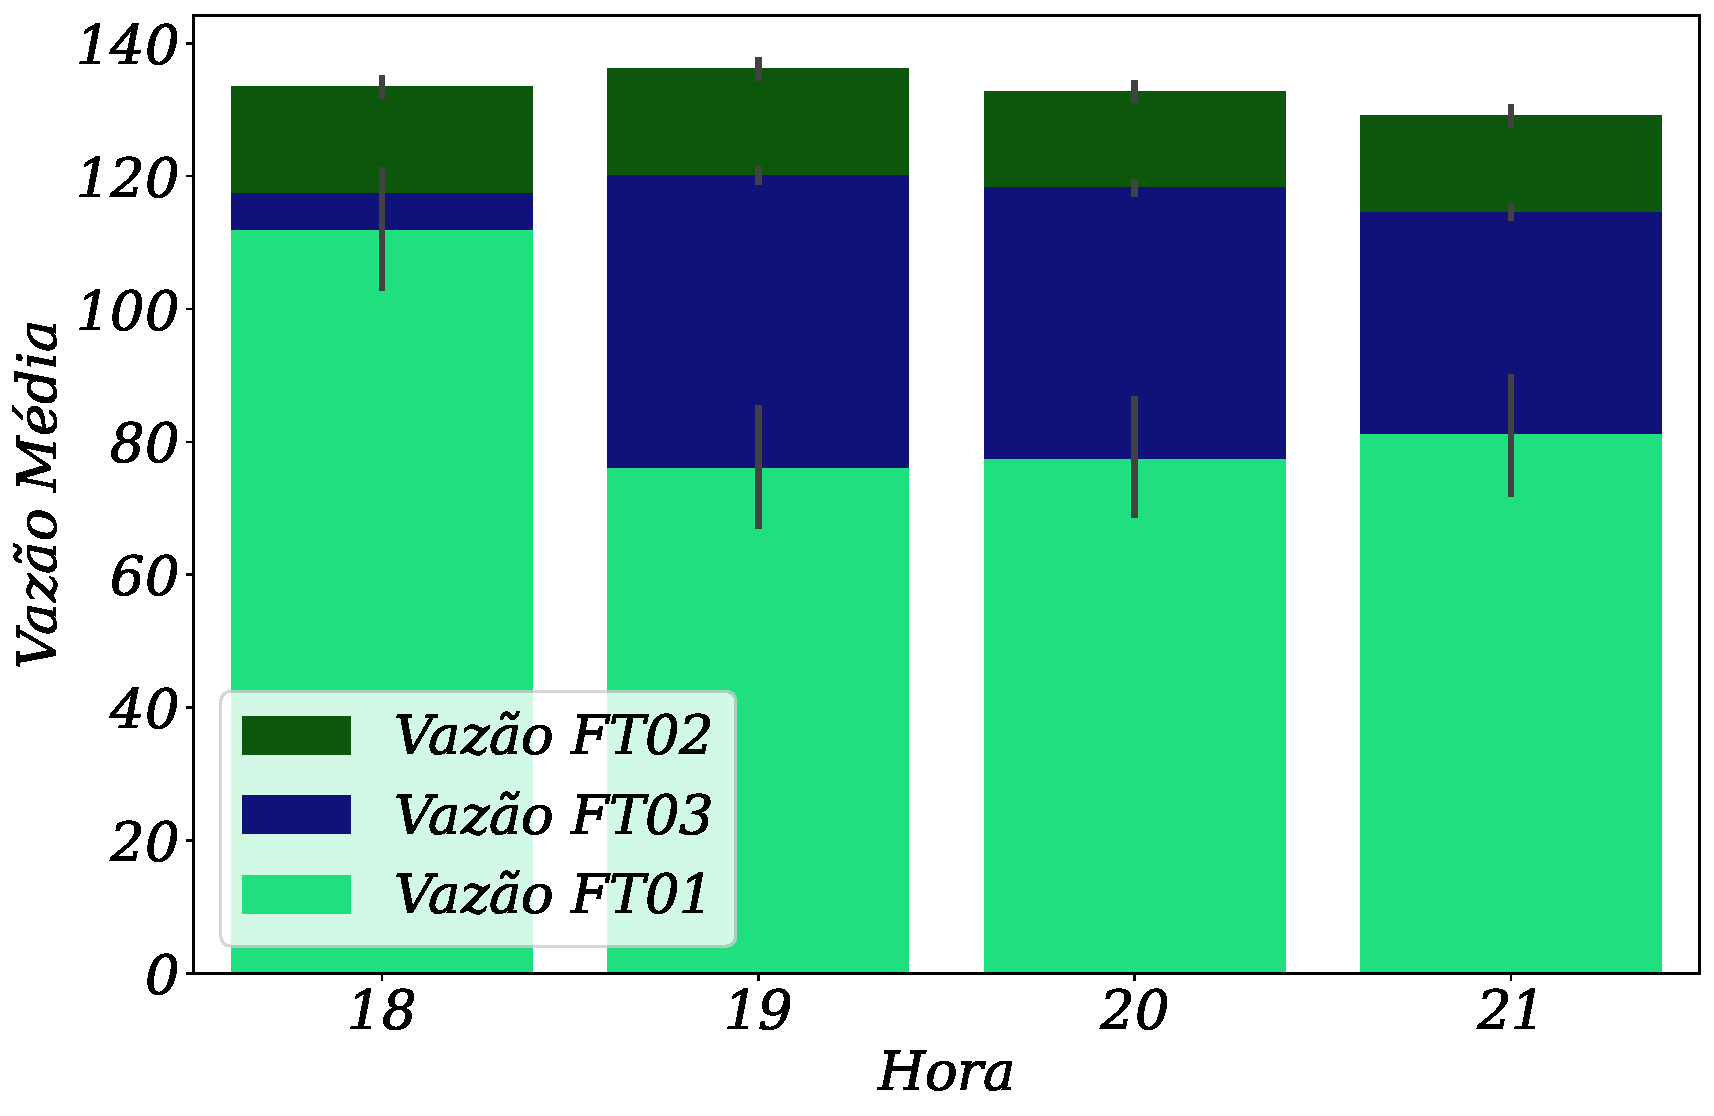
\includegraphics[width=0.7\linewidth]{Resultados/Figuras/grafico-barras-demanda}
	
	\label{fig:grafico-barras-demanda}
	
	
\end{figure}

A Tabela \ref{tb:dem} apresenta os resultados para as três variáveis estudadas: vazão de entrada -- FT01, vazão de gravidade -- FT02 e vazão de recalque -- FT03.
Os resultados destacam os horários específicos em que cada variável apresentou maior demanda dentro do intervalo das 18h às 21h, fornecendo importantes para o planejamento e gerenciamento adequado do sistema. A Tabela \ref{tb:dem} resume essas informações.



\begin{table}[!htb]
	\centering
	\caption{Demanda de água}\label{tb:dem}
	\begin{tabular}{@{}ccc@{}}
		\toprule
		\textbf{Vazões}         & \textbf{Horário de Maior Demanda} & \textbf{Demanda} \\ \midrule
		Entrada -- FT01   & 2020/10/08 21:00:00               & $383,87 \ m^3/h$                   \\
		Gravidade -- FT02 & 2020/10/20 18:00:00               & $326,17 \ m^3/h$                    \\
		Recalque -- FT03  & 2020/11/26 19:00:00               & $194,35 \ m^3/h$                    \\ \bottomrule
	\end{tabular}
	
	
\end{table}

Durante as horas de pico, é necessário que o nível do reservatório esteja mantido dentro na média de $3.9005 \ m^3$ para evitar o acionamento das bombas. Manter o nível do reservatório dentro dessa faixa permitirá que o sistema opere de forma eficiente, atendendo à demanda de água sem a necessidade de acionar as bombas.

É importante destacar que a vazão de recalque exerce um impacto significativo no nível do reservatório em comparação com as outras vazões. Essa diferença se deve ao fato de que a vazão de recalque está diretamente relacionada à injeção de água no reservatório por meio da bomba localizada próxima à sua base. Em contraste, as demais vazões possuem alguns valores ausentes, o que limita sua influência na análise geral do sistema.







